\documentclass[../main.tex]{subfiles}
\begin{document}
\section{Experiment Design} \label{method:experiments}
\note{need to double check that these are actually normally distributed!!}
\begin{itemize}[nosep]
    \item \note{medium instead of mode}
    \item \note{box and whisker plots}
    \item \note{mann whitney u test for significance}
\end{itemize}

\note{Include text explaining how the win-rate matrix works and how the results will be analysed (check the learning from learners paper)}

The ideas of luck and skill are difficult to quantify together. One way to try and eliminate the effects of chance is to run simulations over many thousands of games \cite{guo_distinguishing_2019}. Allowing us to gain a truer measure of skill. 

In order to see the effects luck has on the game it is possible to synthesise events which have a positive impact on the player but may be unlikely to occur. To investigate this idea I propose two sets of experiments, the first looks at the effect of starting a game, and the second at the effect of a player's starting hand.

\subsection{The effect of going first} \label{method:going-first}
In Yaniv the starting order is predetermined, either randomly at the start of an overall game or the winner of the previous round starts. Win streaks are fairly common in the overall game, where a player will continue to win many rounds in a row, which begs the question; how much better is it to start a round? 

\subsubsection{Hypothesis 1}
\begin{displayquote}
Going first increases the likelihood of winning the game.
\end{displayquote}

The first card that is turned over in the game is the top card of the deck after dealing the hands. That means its a random card which is more likely to be desirable than what your opponent will discard, given a players propensity to hold on to low cards. So just how much advantage is gained by having the choice of the first card?

In order to test this I used the rule based agents developed in \autoref{method:rule_agents} and the same environment used to generate \autoref{tab:rules-winrates} but with the starting player fixed over the tournament.

For each combination of the heuristic agents set up a tournament to simulate games. Fix the starting player to the first agent, simulate 10000 games, then fix the starting player to the second agent and simulate another 10000 games. For the case when the agent plays itself, it is only necessary to simulate one set of games with the starting player fixed. The win-rate of the starting player is then recorded. The results are shown in \autoref{tab:rule-wr-going-first}, along with the increases in performance over \autoref{tab:rules-winrates} shown in brackets.

\begin{table}[]
\centering
\begin{tabular}{@{}llll@{}}
             & Random & Novice & Intermediate \\
Random       & 0.0655 (\minus0.0019) & 0.0186 (\pos0.0035) & 0.0111 (\pos0.0000)  \\
Novice       & 0.9414 (\minus0.0003) & 0.5149 (\pos0.0352) & 0.3421 (\pos0.0190)  \\
Intermediate & 0.9865 (\pos0.0023)   & 0.6921 (\pos0.0175) & 0.5206 (\pos0.0253)    
\end{tabular}
\caption{Win-rate matrix for rule based agents when player 0 is fixed as the starting player. Averaged over 10000 games per pairing. Row vs. Column, the agent in the row is goes first. Increase over \autoref{tab:rules-winrates} shown in brackets.}
\label{tab:rule-wr-going-first}
\end{table}

\note{Need to repeat \autoref{tab:rule-wr-going-first} and \ref{tab:rules-winrates} with significantly more data points. Should be able to parallelize it with ray}


\subsubsection{Hypothesis 2}
\begin{displayquote}
As an agents skill increases the effect of going first decreases. 
\end{displayquote}

In order to test this hypothesis I use the RL model's saved policies as a measure of increasing skill. Every 10th training iteration the RL model saves the current version of its policy. Using these policy snapshots its able to run experiments over the RL agents training life, which simulates the idea of getting better. \autoref{fig:model_vs_rules} clearly shows the increase in skill over training iteration against the rule based agents. 

At each saved model 10,000 games are simulated with player 0 going first each time. The win rate of player 0 at each model is plotted on \autoref{fig:win-rate-going-first}.

\begin{figure}
    \centering
    \begin{subfigure}[t]{0.49\textwidth}
        \centering
        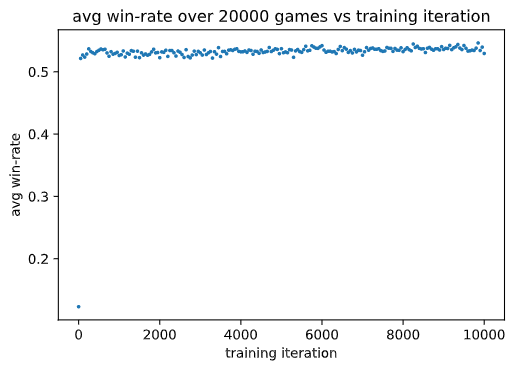
\includegraphics[width=\textwidth,keepaspectratio]{images/results/going_first_over_time.png}
        \caption{Win rate vs Training Iteration in self play when the agent going first is fixed. Every 100th training iteration using 50000.}
        \label{fig:win-rate-going-first}
    \end{subfigure}
    \hfill
    \begin{subfigure}[t]{0.49\textwidth}
        \centering
        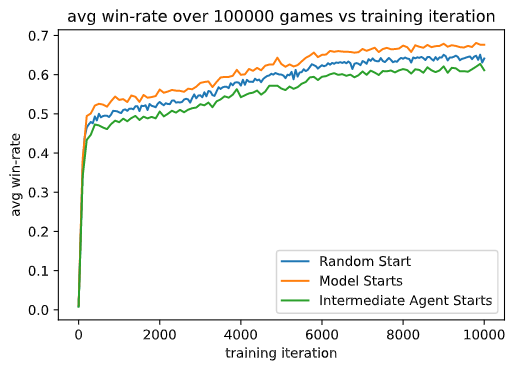
\includegraphics[width=\textwidth,keepaspectratio]{images/results/winrate_vs_int_going_first.png}
        \caption{Win-rate for the model verses the intermediate agent. }
        \label{fig:win-rate-vs-int-going-first}
    \end{subfigure}
    \caption{Going first over training iteration}
    \label{fig:going-first-over-time}
\end{figure}

\subsection{The effect of starting hands}
There are \numprint{2598960} possible 5 card hand configurations. Some of these are better to start with than others. As in poker Yaniv hands can be broken down into classes, based on what they contain, they are detailed along with their frequency in \autoref{tab:hand-classes}. 

Likewise, each starting hand can be scored using the Yaniv rules described in \autoref{intro:rules}. \autoref{fig:startinghand-probs} shows the probability of being dealt a hand of a certain score.

\begin{table}[]
\centering
\begin{tabular}{@{}llll@{}}
\toprule
Class & Description                           & Example        & Frequency \\ \midrule
5S    & 5 card straight                       & C2 C3 C4 C5 C6 & 36        \\
4K    & 4 of a kind                           & C2 H2 S2 D2 C7 & 624       \\
4S    & 4 card straight                       & C2 C3 C4 C5 D4 & 1848      \\
3S2K  & 3 card straight and a pair            & C2 C3 C4 D2 D2 & 2796      \\
3K2K  & Full house                            & C2 D2 H2 S4 H4 & 3744      \\
3S    & 3 card straight                       & C2 C3 C4 H5 S3 & 45144     \\
3K    & 3 of a kind                           & C2 D2 H2 S6 H5 & 54516     \\
2K2K  & Two pair                              & C2 D2 H4 S4 H7 & 2376      \\
2K    & Pair                                  & D7 C7 H2 D6 H3 & 1202604   \\
X     & High Card                             & D7 S9 H2 C5 D3 & 1287648   \\ \bottomrule
\end{tabular}
\caption{Yaniv hand classes}
\label{tab:hand-classes}
\end{table}

\subsubsection{Hypothesis 1}
\begin{displayquote}
Starting with a lower hand score will increase your chances of winning. 
\end{displayquote}

There is a clear advantage to starting with a hand score below 8; it means you can call Yaniv immediately. There are 32 5-card hand combinations which score below 8 which means if you're dealt one there's a 99.9988\% chance that  your opponent has a score >8 which means you can call the game and will likely win. 

Since the goal in Yaniv is to reduce the number of points in your hand to less than 8 it follows that starting with fewer points in your hand will increase your chances of winning. To test this idea I have simulated games where the starting hand of one player is forced to be of a certain score. I used one RL agent to make decisions for both players. \numprint{20000} games were simulated per starting hand score. Results in \autoref{fig:startinghand-winrates}.

\begin{figure}
    \centering
    \begin{subfigure}[t]{0.49\textwidth}
        \centering
        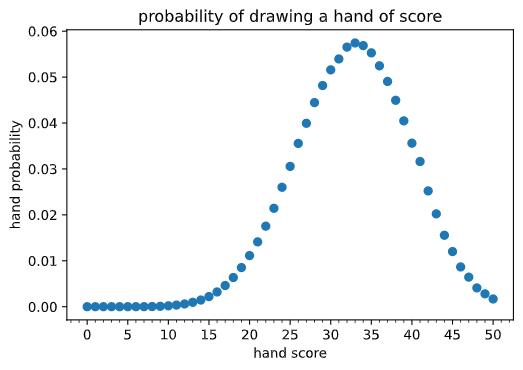
\includegraphics[width=\textwidth,keepaspectratio]{images/results/handscores.png}
        \caption{Frequency of 5 card hand combinations which score. Note that the lowest possible hand score is 6 (4 aces and a two).}
        \label{fig:startinghand-probs}
    \end{subfigure}
    \hfill
    \begin{subfigure}[t]{0.49\textwidth}
        \centering
        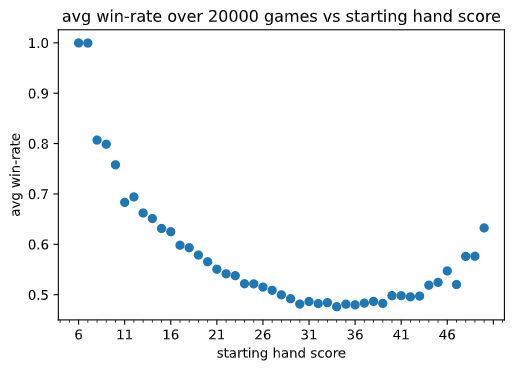
\includegraphics[width=\textwidth,keepaspectratio]{images/results/winrate_handscore.png}
        \caption{Win-rate for given starting hand score.}
        \label{fig:startinghand-winrates}
    \end{subfigure}
    \caption{Hand score results.}
    \label{fig:my_label}
\end{figure}


\subsubsection{Hypothesis 2}
\begin{displayquote}
Starting with a larger legal discard combination combination in your hand will increase your chances of winning.
\end{displayquote}

One of the key strategies in Yaniv is to collect combinations of cards, so that you can discard multiple cards at once. Each time you discard you only pick up one card, so discarding multiple cards is an efficient way to reduce your hand score. Starting with a combination in your hand is a bonus as it means you're immediately able to reduce the number of cards in your hand.

The aim of hypothesis 2 is to test the advantage that starting a round with a hand of a specific type gives you. 

In order to test this I used both intermediate agent and RL Models. The first thing to do is determine the influance starting hand has during self-play. This eliminates the difference in skill between two agents. For each hand class simulate a number of games where the starting hand of player 0 is sampled from the current hand class, while player 1's hand is sampled randomly from the remaining deck. The results of this can be seen in \autoref{fig:handclass-vs-self}. 

Next it is useful to do the same experiment but with different opponents. \autoref{fig:handclass-int-vs-model} shows the results of the intermediate model vs the 10,000th iteration of the RL model. The experiment is conducted in the same way but for each hand class both the agents get a turn at sampling from the class. The aim of this is to show whether an agent can become more skilled at defending against certain unfair advantages. 

\begin{figure}
    \centering
    \begin{subfigure}[t]{0.49\textwidth}
        \centering
        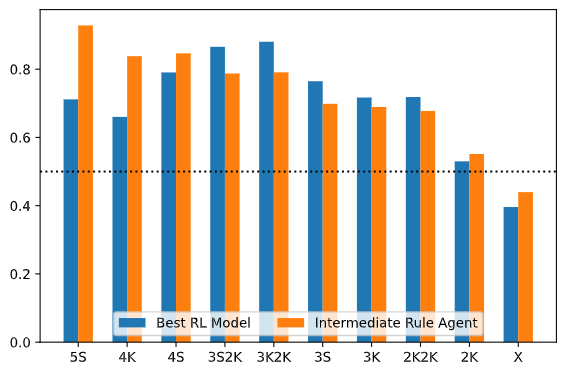
\includegraphics[width=\textwidth,keepaspectratio]{images/results/handclasses.png}
        \caption{Win rates for each handclass. Agents playing against them selves.}
        \label{fig:handclass-vs-self}
    \end{subfigure}
    \hfill
    \begin{subfigure}[t]{0.49\textwidth}
        \centering
        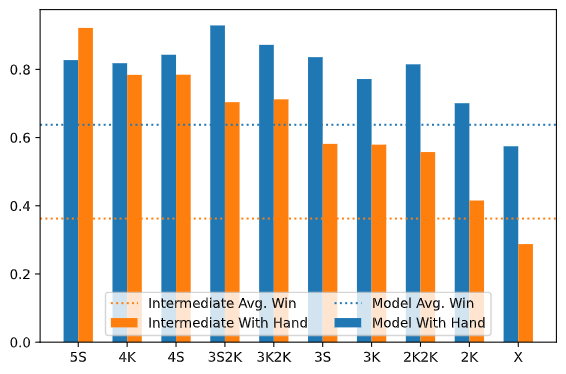
\includegraphics[width=\textwidth,keepaspectratio]{images/results/handclasses_model_vs_rules.png}
        \caption{Hand class win rates for Model vs Intermediate. Along with the base line win-rate for each (random hands).}
        \label{fig:handclass-int-vs-model}
    \end{subfigure}
    \label{fig:handclass-winrates}
    \caption{Win rates for different hand classes. Uses the intermediate rule agent and the 10,000th iteration of the RL model. Averaged over 100,000 games. The opponent's starting hand is sampled from the deck after generating the starting hand of the given class.}
\end{figure}

\subsubsection{Hypothesis 3}
\begin{displayquote}
As an agents skill increases, its ability to exploit better starting hands increases.
\end{displayquote}

As an agents skill increases its ability to exploit \textit{lucky} events should increase, but so should its ability to negate the effects of a lucky opponent. By forcing events which have a clearly positive impact (from hypothesis 2) I aim to see the effect skill has on neutralising luck. 

\begin{itemize}[noitemsep]
    \item \textbf{Independent Variables}: Starting hand class, model iteration
    \item \textbf{Dependent Variables}: Avg. Win rate
    \item \textbf{Control Variables}: Number of simulated games, starting player, opponent starting hand
\end{itemize}

The experiment design is simple and is as follows. For each model and starting hand class run a series of game simulations where the model is used as the policy for both players. The starting player is chosen randomly per game, and the opponents hand is sampled from the deck after a hand is sampled from the hand class. Results in \autoref{fig:handclass-overtime}

\begin{figure}
    \centering
    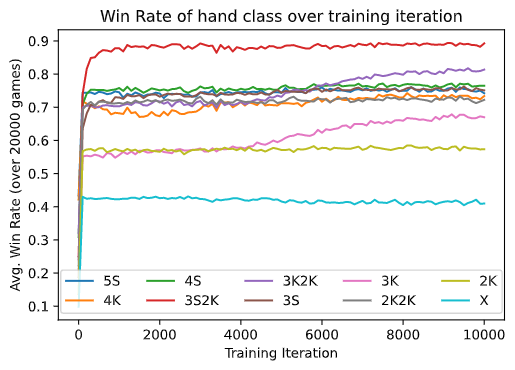
\includegraphics[width=\textwidth,keepaspectratio]{images/results/handclassovertime.png}
    \caption{Win-rate for given class over training iterations.}
    \label{fig:handclass-overtime}
\end{figure}
\end{document}